\documentclass[12pt,a4paper]{article}
\usepackage[utf8]{inputenc}
\usepackage{graphicx}
\usepackage{color}
\usepackage[boxruled, linesnumbered]{algorithm2e}
\usepackage{caption}
\usepackage{subcaption}

\title{CmpE321}
\author{Mustafa Enes Çakır}
\date{July 2017}


\begin{document}

\begin{titlepage}

\newcommand{\HRule}{\rule{\linewidth}{0.5mm}}

\center % Center everything on the page

%----------------------------------------------------------------------------------------
%   HEADING SECTIONS
%----------------------------------------------------------------------------------------

\textsc{\LARGE BOĞAZİÇİ UNIVERSITY}\\[1.5cm] % Name of your university/college
\textbf{\Large CMPE 321}\\[0.5cm] % Major heading such as course name
\textsc{\large PROJECT 2}\\[2cm] % Minor heading such as course title
\textsc{\large Summer 2017}\\[3cm] % Minor heading such as course title

%----------------------------------------------------------------------------------------
%   TITLE SECTION
%----------------------------------------------------------------------------------------

\HRule \\[0.4cm]
{ \huge \bfseries Storage Manager Implementation}\\[0.4cm] % Title of your document
\HRule \\[4cm]

%----------------------------------------------------------------------------------------
%   AUTHOR SECTION
%----------------------------------------------------------------------------------------

\Large Mustafa Enes ÇAKIR \\ [2cm] % Your name

%----------------------------------------------------------------------------------------
%   DATE SECTION
%----------------------------------------------------------------------------------------

{\large July 27, 2017}\\[2cm] % Date, change the \today to a set date if you want to be precise
\vfill % Fill the rest of the page with whitespace
\end{titlepage}

\tableofcontents{}

\break

\section{Introduction}
    A storage manager is a program that controls how the memory will be used to save data to increase the efficiency of a system.
    In the previous project, I had designed a Storage Manager System without error checking. While I was implementing the design, some things aren't fit to blueprints. I changed some data structures. This document consists of the implementation details for a simple database management system, including changes from previous project, sample outputs screenshots.
    I implemented it in Java.
\section{Changes from the Initial Design}
    I add some attributes to data structures for accessing easily. Furthermore, I add a \emph{Disc Directory} page for simulating virtual hard disc files.
    This design contains three main components which are Disc Directory, System Catalogue and  Data Files.
    \subsection{Disc Directory}
        Disc directory is responsible for storing the file address. Also it keeps last free address. \\

        \begin{table}[h!]
                \begin{center}
                    \begin{tabular}{ | c | c | c | c | }
                    \hline
                    0 & 1 & 2 & 3 \\
                    \hline
                    4 & 5 & 6 & 7 \\
                    \hline
                    8 & 9 & 10 & 11 \\
                    \hline
                    12 & 13 & 14 & 15 \\
                    \hline
                    \end{tabular}
                \end{center}
            \caption{Hard Disc Abstraction}
            \label{table:1}
        \end{table}

        \begin{table}[h!]
                \begin{center}
                    \begin{tabular}{ | c | c| }
                    \hline
                    File Name & Address \\
                    \hline
                    \hline
                    Free Space & 5 \\
                    \hline
                    SysCat.txt & 1 \\
                    \hline
                    Dog.txt & 2 \\
                    \hline
                    Cat.txt & 4 \\
                    \hline
                    \end{tabular}
                \end{center}
            \caption{Disc Directory}
            \label{table:2}
        \end{table}

    \subsection{System Catalogue}
        System catalogue is responsible for storing the metadata. It's a blueprint for datas. It has multiple pages. Each record has a fixed size. I add two more fields to page headers and one more to record header. Each type has 10 fields. Therefore, the space of each record in the system catalog is 134 bytes. So 10 data type records can be stored in a page.
        \begin{itemize}
          \item Page Header (13 bytes)
            \begin{itemize}
                \item Page ID (4 bytes)
                \item Pointer to Next Page (4 bytes)
                \item \# of Records (4 bytes)
                \item isEmpty (1 byte)
            \end{itemize}
          \item Record (133 bytes)
            \begin{itemize}
                 \item Record Header (14 bytes)
                    \begin{itemize}
                        \item Type Name (12 bytes)
                        \item \# of Fields (1 byte)
                        \item isEmpty (1 byte)
                    \end{itemize}
                 \item Field Names (10 x 12 = 120 bytes)
            \end{itemize}
        \end{itemize}

        \begin{table}[h!]
                \begin{center}
                    \begin{tabular}{ | c | c | c || c | c | c | }
                    \hline
                    \multicolumn{1}{||c|}{Page ID} &
                    \multicolumn{2}{|c|}{Pointer to Next Page} &
                    \multicolumn{2}{|c|}{\# of Records} &
                    \multicolumn{1}{|c||}{isEmpty} \\
                    \hline
                    \hline
                    Type Name 1 & \# of Fields & isEmpty & Field Name 1 & ... & Field Name 10 \\
                    \hline
                    Type Name 2 & \# of Fields & isEmpty & Field Name 1 & ... & Field Name 10 \\
                    \hline
                    ... & ... & ... & ... & ... & ... \\
                    \hline
                    Type Name 10 & \# of Fields & isEmpty & Field Name 1 & ... & Field Name 10 \\
                    \hline
                    \end{tabular}
                \end{center}
            \caption{a Page of a System Catalogue \emph{(Starting with the Page Header)}}
            \label{table:3}
        \end{table}

    \subsection{Data Files}
        Data files store actual datas. I didn'd change my data files. In this storage manager system, data files are separated into the number of types. Each data file can store one type of record and is named with that type. \emph{"hamster.txt"} can store only the records of type \emph{hamster} for example. These records can be thought as instances of a type in the system catalog. Therefore the fields of the records are actual values. Here, all the values are integer. A record in a data file has a space of 45 bytes. Each page in a data file can store 30 records at most.
        \subsubsection{Pages}
            Page headers store information about the specific page it belongs to.
            \begin{itemize}
              \item Page Header (13 bytes)
                \begin{itemize}
                     \item Page ID (4 bytes)
                    \item Pointer to Next Page (4 bytes)
                     \item \# of Records (4 bytes)
                     \item isEmpty (1 byte)
                \end{itemize}
              \item Records (a Record = 45 bytes)
            \end{itemize}
        \subsubsection{Records}
            \begin{itemize}
              \item Record Header (5 bytes)
                \begin{itemize}
                     \item Record ID (4 bytes)
                    \item isEmpty (1 bytes)
                \end{itemize}
              \item Fields (10 x 4 = 40 bytes)
            \end{itemize}

        \begin{table}[h!]
            \begin{center}
                \begin{tabular}{ | c | c | c | c | c | c | }
                \hline
                    \multicolumn{1}{||c|}{Page ID} &
                    \multicolumn{2}{|c|}{Pointer to Next Page} &
                    \multicolumn{2}{|c|}{\# of Records} &
                    \multicolumn{1}{|c||}{isEmpty} \\
                \hline
                \hline
                Record ID 1 & isEmpty & Field 1 & Field 2 & ... & Field 10 \\
                \hline
                Record ID 2 & isEmpty & Field 1 & Field 2 & ... & Field 10 \\
                \hline
                ... & ... & ... & ... & ... & ... \\
                \hline
                Record ID 30 & isEmpty & Field 1 & Field 2 & ... & Field 10 \\
                \hline
                \end{tabular}
            \end{center}
    \caption{Page of a Data File \emph{(Starting with the Page Header)}}
    \label{table:4}
    \end{table}

\section{Sample Outputs}
\hfill
\begin{figure}
\centering
\begin{subfigure}{.5\textwidth}
  \centering
  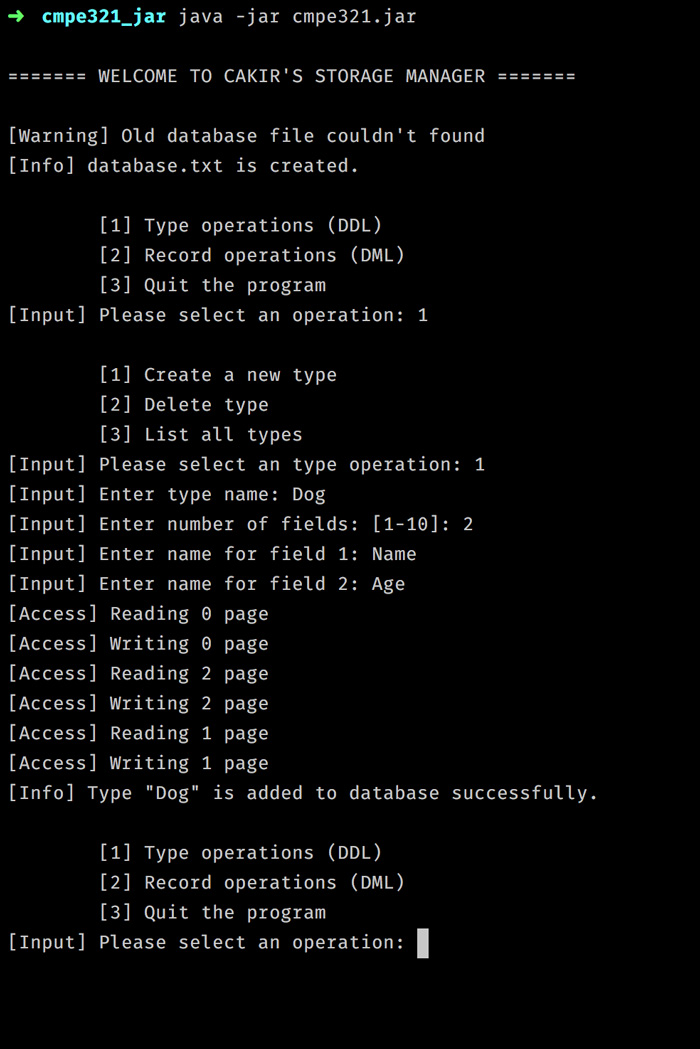
\includegraphics[width=.90\linewidth]{ss1.jpg}
  \caption{Create type}
  \label{fig:sub1}
\end{subfigure}%
\begin{subfigure}{.5\textwidth}
  \centering
  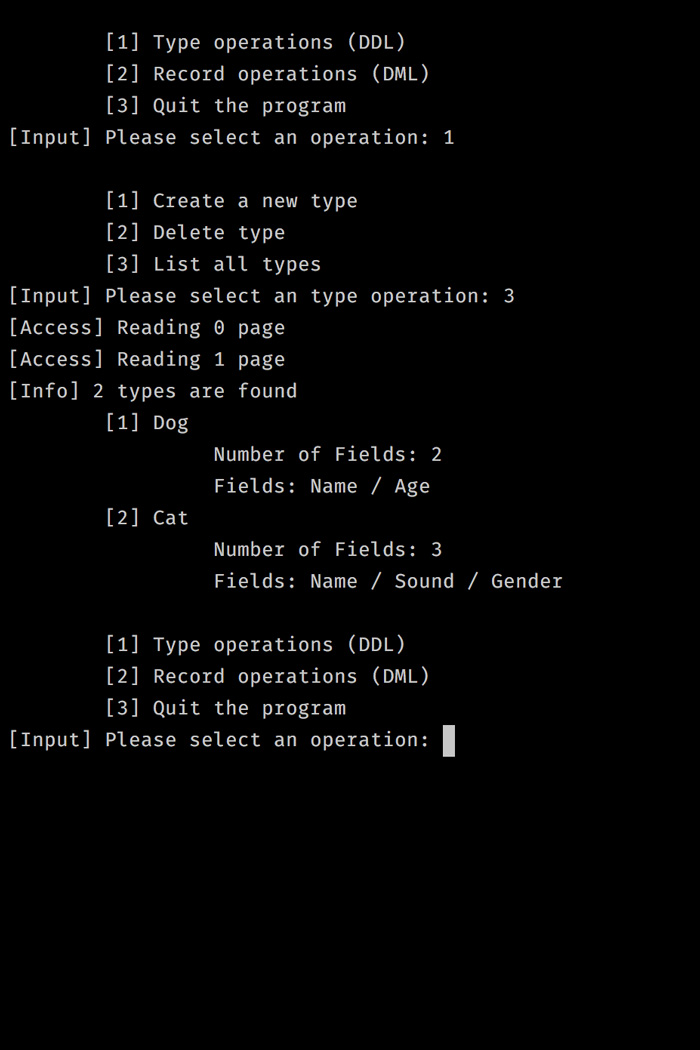
\includegraphics[width=.90\linewidth]{ss2.jpg}
  \caption{List all types}
  \label{fig:sub2}
\end{subfigure}
\end{figure}

\begin{figure}
\centering
\begin{subfigure}{.5\textwidth}
  \centering
  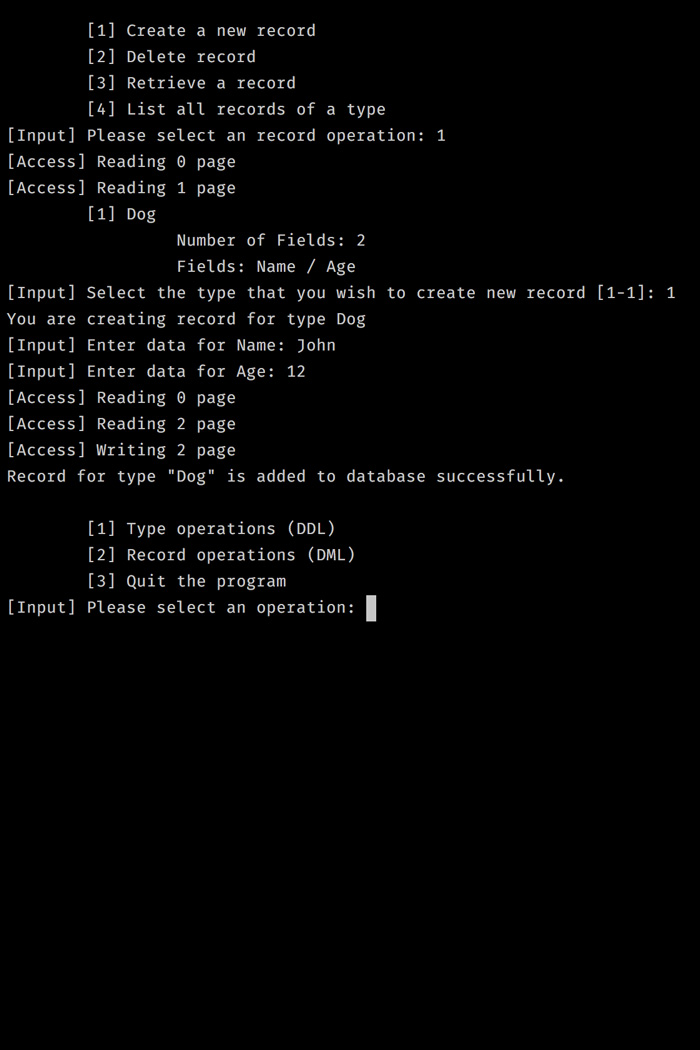
\includegraphics[width=.90\linewidth]{ss3.jpg}
  \caption{Create record}
  \label{fig:sub3}
\end{subfigure}%
\begin{subfigure}{.5\textwidth}
  \centering
  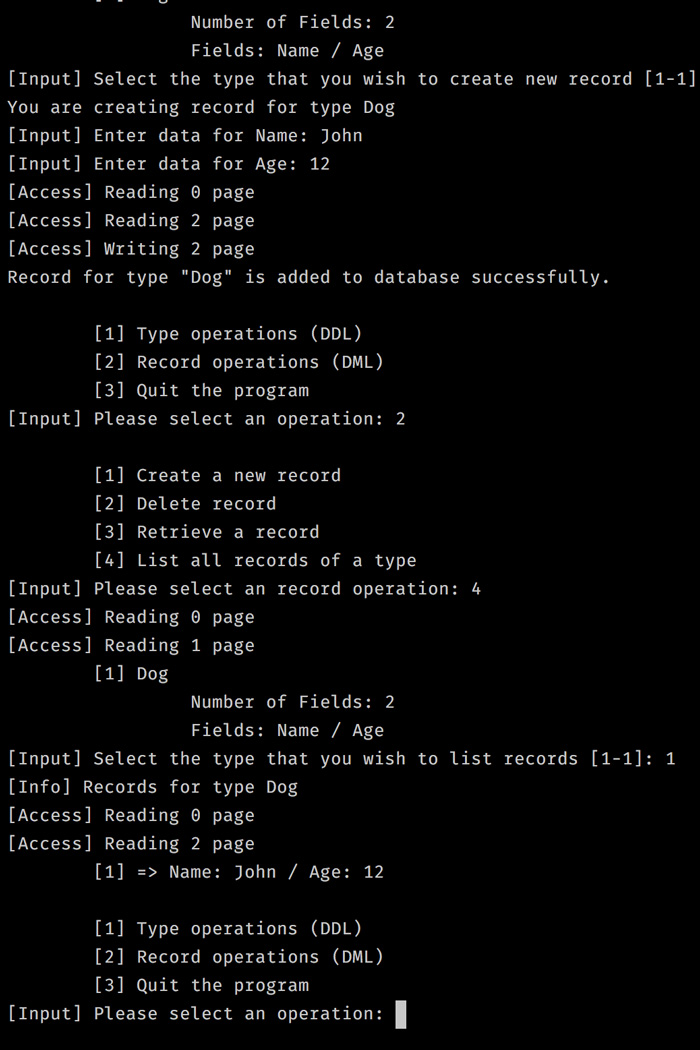
\includegraphics[width=.90\linewidth]{ss4.jpg}
  \caption{List all records of a type}
  \label{fig:sub4}
\end{subfigure}
\end{figure}

\section{Conclusions \& Assessment}
    In this experience, I see design and implementation always don't fit perfectly. I need to change some data structures.
    In this documentation a storage manager design is proposed where size of each
structure is fixed. This creates an inefficiency in terms of memory usage while
it makes the storage manager easier to implement. I allocated 1400 Bytes space for pages however the system only uses 1363 Bytes, this is done for Reliability.  Also note that, the pages
and records are inserted to storage manager linearly without any specific order. This makes searching slower whereas it makes
insertion faster. It's faster when listing records. \\
    This restricts the user to some extent, however it makes the storage manager
faster since the length controls are unnecessary, no checking for identical key is
needed. \\
    \\
    To sum up, this implementation has its own ups and downs just like every implementation.
    Since it is kept as a simple one, it is easy to modify and improve. Hence,
implementing it would also be easier with necessary modifications that can be
realized on the run.
\end{document}
